\documentclass[11pt,a4paper]{article}

\usepackage[utf8]{inputenc}
\usepackage[T1]{fontenc}
\usepackage[french]{babel}
\usepackage{lmodern}
\usepackage[margin=2.4cm]{geometry}
\usepackage{graphicx}
\usepackage{booktabs}
\usepackage{amsmath, amssymb}
\usepackage{float}
\usepackage{xcolor}
\usepackage{caption}
\usepackage{textcomp}
\usepackage[colorlinks=true, linkcolor=blue!50!black, urlcolor=blue!50!black]{hyperref}

\graphicspath{{../figures/}}

% Tolérance d'espacement pour éviter les débordements
% causés par les identifiants \texttt insécables
\emergencystretch=3em

\definecolor{accentblue}{HTML}{1F77B4}
\definecolor{accentred}{HTML}{D62728}

\newcommand{\eur}{\texteuro}

\title{
    \vspace{1cm}
    {\Large Tarification automobile en assurance non-vie}\\[0.4cm]
    {\huge \bfseries Modélisation de la prime pure par approches GLM et Machine Learning}\\[0.5cm]
    {\large Fréquence \texttimes{} Sévérité, traitement des sinistres graves et tarification Tweedie\\ sur le portefeuille \texttt{freMTPL}}
    \vspace{1cm}
}
\author{Projet de tarification actuarielle}
\date{Juillet 2026}

\begin{document}

\maketitle
\vfill
\begin{abstract}
\noindent
Ce rapport présente la construction complète d'un tarif de prime pure en assurance automobile (responsabilité civile) sur le portefeuille français \texttt{freMTPL} (413\,169 polices, 16\,181 sinistres). La démarche suit l'approche actuarielle standard de décomposition fréquence \texttimes{} sévérité par modèles linéaires généralisés (GLM Poisson et Gamma), enrichie d'un traitement rigoureux des sinistres graves par écrêtement et chargement, puis confrontée à deux approches de machine learning : une décomposition fréquence \texttimes{} sévérité par gradient boosting (LightGBM) et un modèle Tweedie direct. Les quatre tarifs sont comparés sur des métriques adaptées (déviance de Poisson, indice de Gini, ratio S/P, courbes de lift), et leurs effets sont analysés par relativités, partial dependence et valeurs SHAP. Le GLM reste compétitif face au ML sur ce portefeuille : il conserve le meilleur pouvoir de segmentation (Gini de 0{,}191 contre 0{,}183 pour le ML), tandis que le gradient boosting améliore légèrement la déviance de fréquence. L'analyse met également en évidence deux constats structurants : la sévérité est très peu segmentable au-delà de sa moyenne, et l'exposition du portefeuille est partiellement endogène au sinistre.
\end{abstract}
\vfill
\newpage

\tableofcontents
\newpage

% =====================================================================
\section{Introduction et contexte}
% =====================================================================

La tarification en assurance non-vie repose sur l'estimation de la \emph{prime pure} : l'espérance du coût des sinistres qu'une police générera pendant sa période de couverture. Un tarif doit satisfaire simultanément deux objectifs en tension :

\begin{itemize}
    \item \textbf{l'équilibre technique} : au niveau du portefeuille, la somme des primes doit couvrir la charge de sinistres attendue (ratio Sinistres/Primes proche de 1) ;
    \item \textbf{la segmentation} : à profil de risque différent, prime différente. Un tarif insuffisamment segmenté expose l'assureur à l'antisélection --- les bons risques partent chez un concurrent mieux segmenté, les mauvais restent.
\end{itemize}

Ce projet construit et compare quatre tarifs de prime pure sur un portefeuille automobile français, en suivant une progression méthodologique : modèle GLM classique, enrichissement par un traitement des sinistres graves, puis deux challengers de machine learning. L'objectif n'est pas seulement de produire un tarif, mais de justifier chaque choix de modélisation et d'évaluer honnêtement ce que chaque approche apporte --- ou n'apporte pas.

% =====================================================================
\section{Données}
% =====================================================================

\subsection{Description du portefeuille}

Le jeu de données \texttt{freMTPL} (French Motor Third-Party Liability) décrit un portefeuille de responsabilité civile automobile française observé sur une année. Il se compose de deux tables :

\begin{itemize}
    \item une table de \textbf{polices} (413\,169 lignes) : identifiant, nombre de sinistres (\texttt{ClaimNb}), exposition en années-police (\texttt{Exposure}), et sept variables tarifaires --- puissance du véhicule (\texttt{Power}), âge du véhicule (\texttt{CarAge}), âge du conducteur (\texttt{DriverAge}), marque (\texttt{Brand}), carburant (\texttt{Gas}), région (\texttt{Region}) et densité de population de la commune (\texttt{Density}) ;
    \item une table de \textbf{sinistres} (16\,181 lignes) : identifiant de police et montant du sinistre.
\end{itemize}

\begin{table}[H]
\centering
\caption{Chiffres clés du portefeuille}
\begin{tabular}{lr}
\toprule
Nombre de polices & 413\,169 \\
Polices sinistrées & 15\,390 (3{,}7\,\%) \\
Nombre de sinistres & 16\,181 \\
Charge totale & 34{,}5~M\eur \\
Exposition totale & 231\,780 années-police \\
Fréquence globale & 0{,}0698 sinistre / année-police \\
Sévérité moyenne & 2\,088~\eur \\
Sévérité médiane & 1\,156~\eur \\
Sinistre maximal & 2\,04~M\eur \\
\bottomrule
\end{tabular}
\end{table}

L'écart considérable entre sévérité médiane (1\,156~\eur) et moyenne (2\,088~\eur), et un maximum à plus de 2~M\eur, signalent d'emblée une queue de distribution très épaisse : ce constat motivera le traitement dédié des sinistres graves (section~\ref{sec:graves}).

\subsection{Qualité des données et retraitements}

Deux retraitements sont appliqués en amont de toute modélisation :

\paragraph{Écrêtement de l'exposition.} 421 polices (0{,}1\,\% du portefeuille) présentent une exposition supérieure à 1 an (jusqu'à 1{,}99), ce qui est physiquement impossible pour des contrats annuels : il s'agit d'une anomalie documentée de ce jeu de données. L'exposition intervenant en offset du modèle de fréquence --- avec un coefficient contraint à 1, donc une confiance totale du modèle --- ces valeurs sont écrêtées à 1, conformément à la pratique de la littérature.

\paragraph{Agrégation des sinistres par police.} Les montants sont agrégés au niveau police (\texttt{ClaimAmount\_total}) et la sévérité moyenne par police est définie comme le rapport de cette charge totale au nombre de sinistres de la police. Cette granularité police (et non sinistre) est une contrainte assumée dont les conséquences sur le traitement des graves sont discutées en section~\ref{sec:graves}.

\subsection{Analyse exploratoire}

L'analyse exploratoire (distributions des variables qualitatives et quantitatives, fréquences par modalité --- figures du dossier \texttt{figures/}) guide directement les choix de préparation des variables :

\begin{itemize}
    \item plusieurs modalités de \texttt{Power}, \texttt{Brand} et \texttt{Region} pèsent moins de 5\,\% de l'exposition : leurs coefficients GLM seraient instables, d'où les regroupements de la section~\ref{sec:prep} ;
    \item la fréquence de sinistre varie nettement selon la densité, l'âge du conducteur et la région, ce qui justifie leur inclusion tarifaire ;
    \item \texttt{Density} est distribuée sur plusieurs ordres de grandeur, d'où sa transformation logarithmique.
\end{itemize}

\begin{figure}[H]
\centering
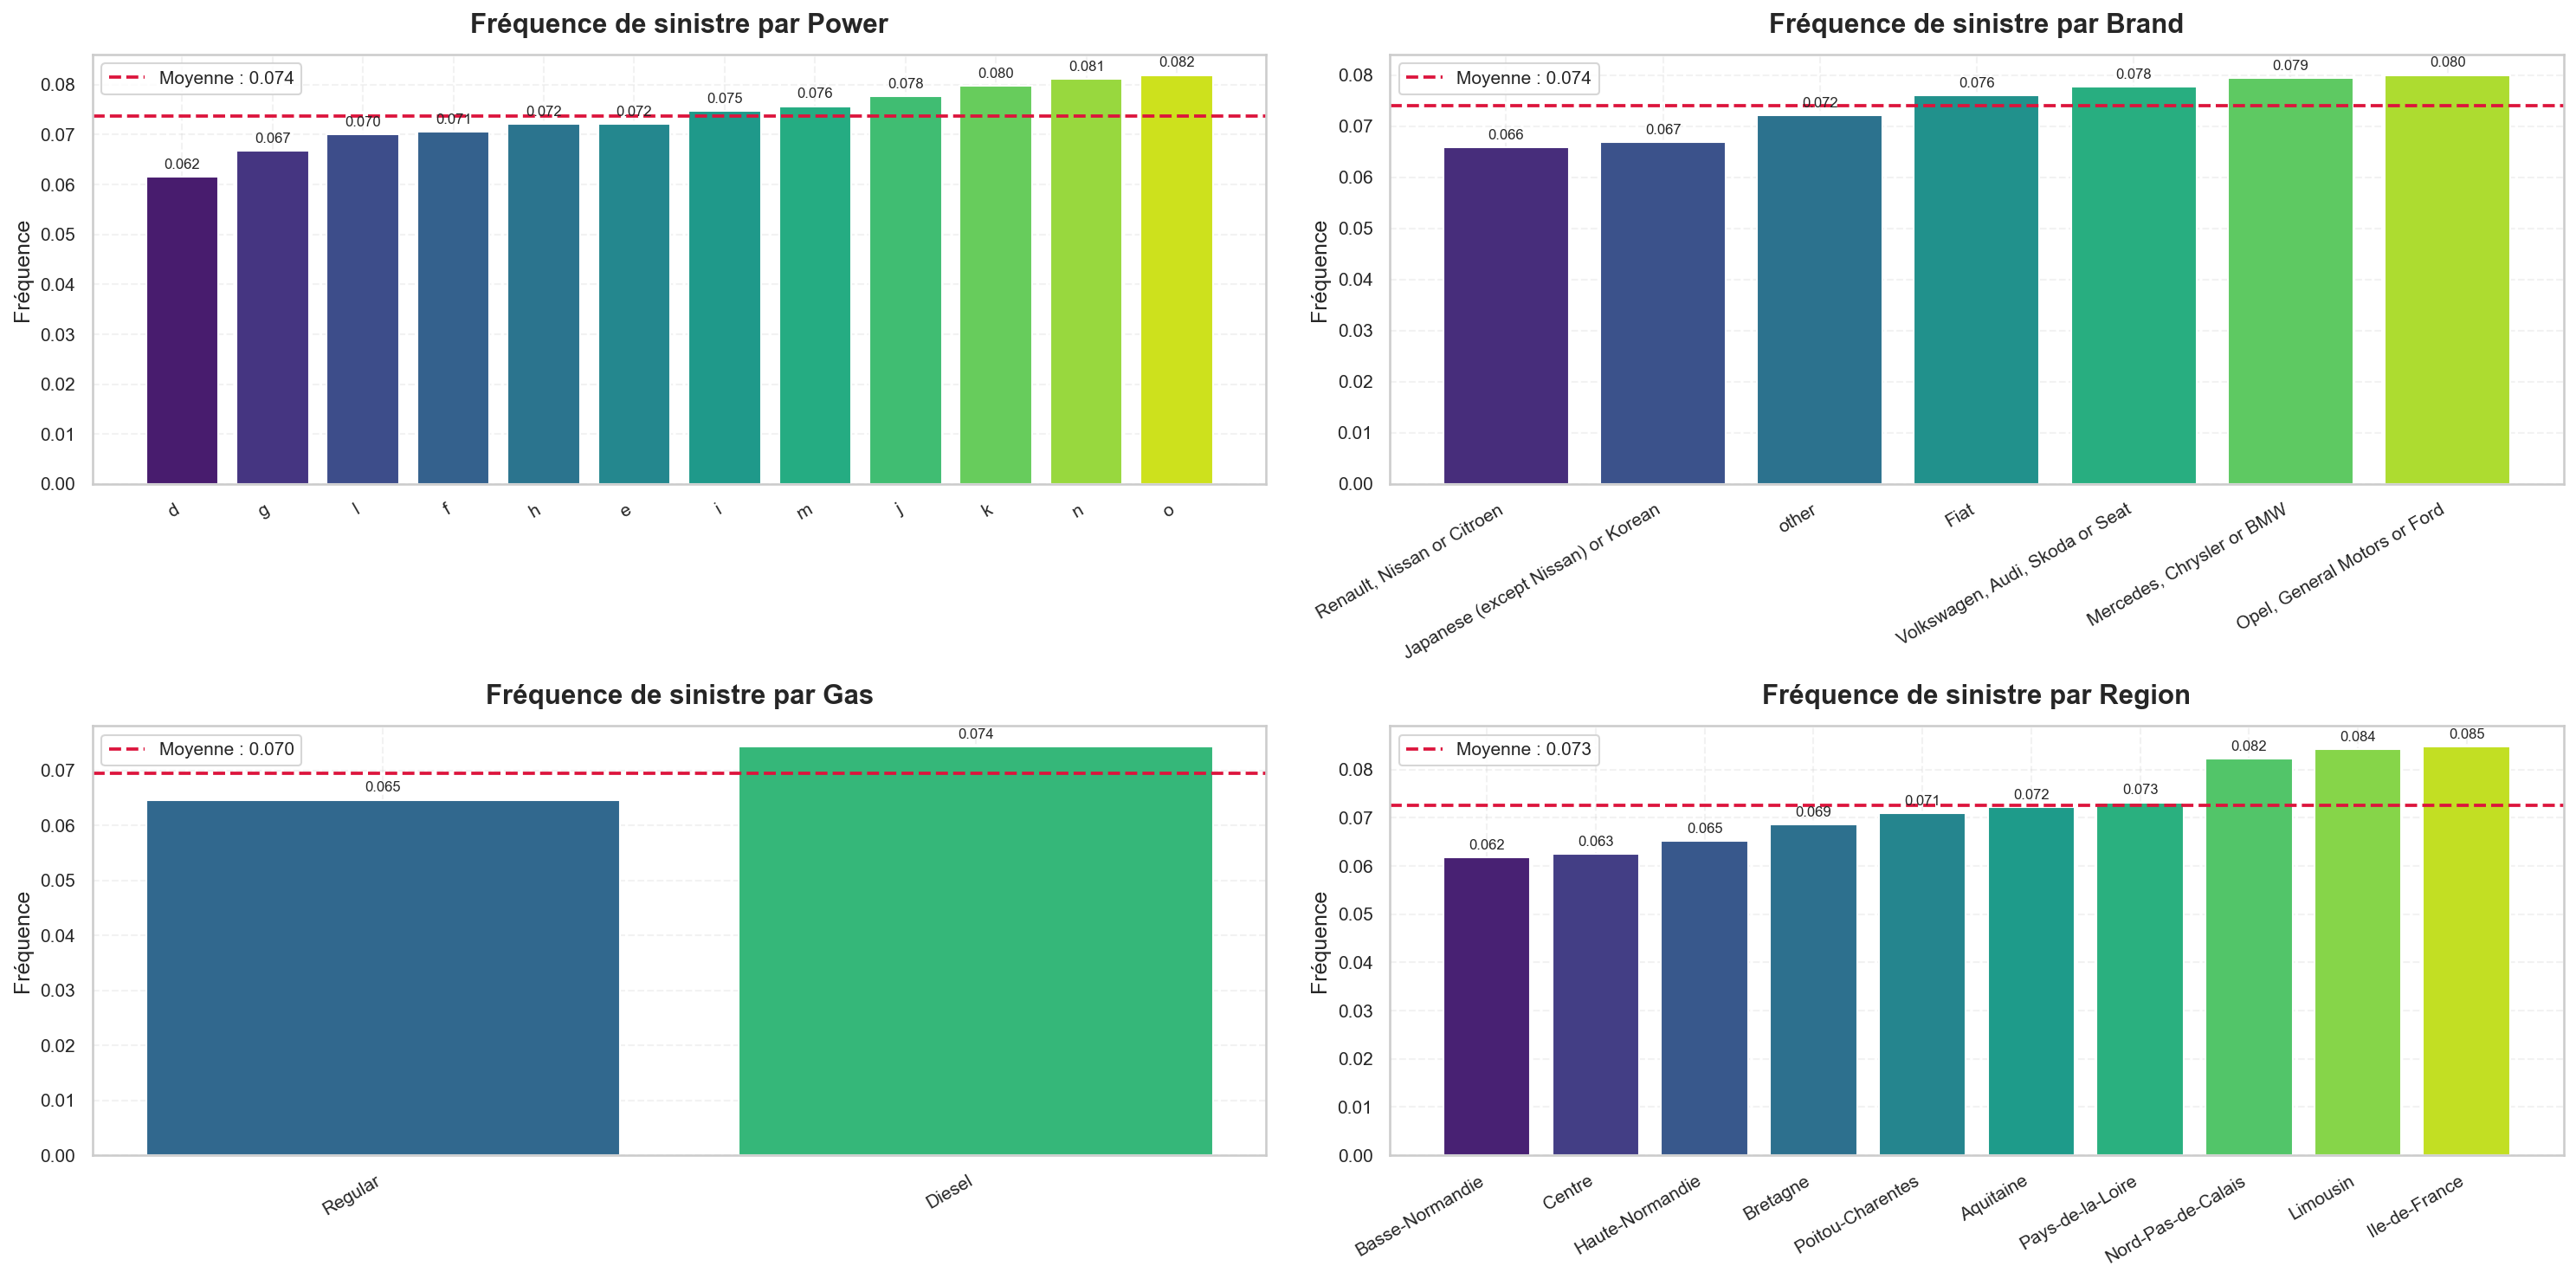
\includegraphics[width=\textwidth]{claim_frequency.png}
\caption{Fréquence de sinistre observée par modalité des variables qualitatives (train).}
\end{figure}

% =====================================================================
\section{Méthodologie générale}
% =====================================================================

\subsection{Décomposition fréquence \texttimes{} sévérité}

L'approche actuarielle standard modélise séparément le nombre de sinistres $N$ et leur coût moyen $S$, sous hypothèse d'indépendance :
\begin{equation}
    \text{Prime pure} \;=\; \mathbb{E}[N] \times \mathbb{E}[S].
\end{equation}

Cette décomposition présente trois avantages : les deux phénomènes obéissent à des lois différentes (comptage vs montant positif asymétrique), leurs déterminants diffèrent (la fréquence est bien plus segmentable que la sévérité, ce que nos résultats confirmeront), et le tarif reste interprétable composante par composante.

\subsection{Modèles linéaires généralisés}

\paragraph{Fréquence : Poisson avec offset.} Le nombre de sinistres est modélisé par un GLM de Poisson avec lien logarithmique et \emph{offset} $\log(\text{Exposure})$ :
\begin{equation}
    N_i \sim \mathcal{P}\bigl(\lambda_i \, e_i\bigr), \qquad
    \log \lambda_i = \beta_0 + \sum_j \beta_j x_{ij},
\end{equation}
où $e_i$ est l'exposition de la police $i$. L'offset garantit que le modèle estime une fréquence \emph{annuelle} $\lambda_i$, l'exposition étant réintégrée mécaniquement en prédiction. Une propriété précieuse du couple Poisson/log est l'\emph{équilibre marginal} : sur le train, la somme des sinistres prédits égale la somme observée, globalement et par modalité de chaque variable du modèle.

\paragraph{Sévérité : Gamma avec lien log et pondération.} Le coût moyen par sinistre est modélisé par un GLM Gamma à lien logarithmique, ajusté sur les seules polices sinistrées. La cible étant une \emph{moyenne} par police, chaque observation est pondérée par son nombre de sinistres (\texttt{var\_weights} $= \texttt{ClaimNb}$) : une moyenne calculée sur 4 sinistres est intrinsèquement plus fiable qu'une moyenne sur un seul. Omettre cette pondération --- erreur fréquente --- revient à accorder le même crédit à toutes les polices sinistrées.

\paragraph{Multiplicativité du tarif.} Le lien logarithmique des deux modèles rend le tarif \emph{multiplicatif} : la prime d'un profil s'obtient en multipliant une prime de référence par les \emph{relativités} $e^{\beta_j}$ de ses modalités. C'est le format standard des grilles tarifaires du marché, directement lisible par un souscripteur.

\subsection{Protocole de validation}

Le portefeuille est scindé en 80\,\% d'apprentissage et 20\,\% de test. Un point de protocole mérite d'être souligné : le découpage de la base de sévérité est \emph{dérivé} du découpage de la base de fréquence via l'identifiant de police. Deux découpages aléatoires indépendants --- solution naïve --- placeraient des polices dans le train du modèle de sévérité \emph{et} dans le test du tarif final, contaminant l'évaluation. Toutes les métriques rapportées ici sont calculées sur des polices jamais vues par aucun des modèles.

% =====================================================================
\section{Préparation des variables tarifaires}
\label{sec:prep}
% =====================================================================

\subsection{Regroupement des modalités}

Les variables qualitatives présentent des modalités trop fines ou trop rares pour une estimation stable. Les regroupements suivent deux critères : la \textbf{proximité des fréquences de sinistre observées} (on ne regroupe que des risques homogènes) et, pour les régions, la \textbf{proximité géographique}.

\paragraph{Puissance.} Les douze niveaux (\texttt{d} à \texttt{o}) sont regroupés en sept classes (\texttt{d}, \texttt{f}, \texttt{h}, \texttt{i\_j\_k}, \texttt{m\_e}, \texttt{l\_o\_g}, \texttt{n}) sur la base de fréquences observées comparables entre niveaux adjacents.

\paragraph{Marque.} Fiat rejoint le groupe Mercedes/Chrysler/BMW (\texttt{MCB\_Fiat}) et la modalité résiduelle \og other \fg{} rejoint Renault/Nissan/Citroën (\texttt{RNC\_other}), là encore sur similarité des fréquences.

\paragraph{Région : double critère fréquence + géographie.} Les dix anciennes régions administratives sont regroupées en quatre zones tarifaires (figure~\ref{fig:regions}). Le regroupement ne s'appuie pas uniquement sur la ressemblance statistique : il privilégie la \emph{contiguïté géographique}, gage de cohérence du zonier (facteurs de risque territoriaux communs : réseau routier, climat, densité du trafic) et de sa robustesse dans le temps.

\begin{itemize}
    \item \textbf{Centre / Bretagne / Normandies} (fréquences 0{,}0630 à 0{,}0693) : bloc contigu du quart nord-ouest, fréquences les plus basses du portefeuille ;
    \item \textbf{Pays-de-la-Loire / Poitou-Charentes / Aquitaine} (0{,}0717 à 0{,}0737) : façade atlantique contiguë, fréquences intermédiaires très homogènes ;
    \item \textbf{Nord-Pas-de-Calais / Limousin} (0{,}0822 pour les deux) : fréquences strictement identiques. Ces deux régions ne sont pas contiguës --- le regroupement est ici purement statistique, assumé pour préserver un effectif suffisant (le Limousin ne pèse que 2\,396 années-police) ;
    \item \textbf{Île-de-France} (0{,}0858) : la fréquence la plus élevée, conservée seule --- son profil de risque (trafic dense, sinistralité matérielle fréquente) et son poids dans le portefeuille justifient une zone dédiée.
\end{itemize}

\begin{figure}[H]
\centering
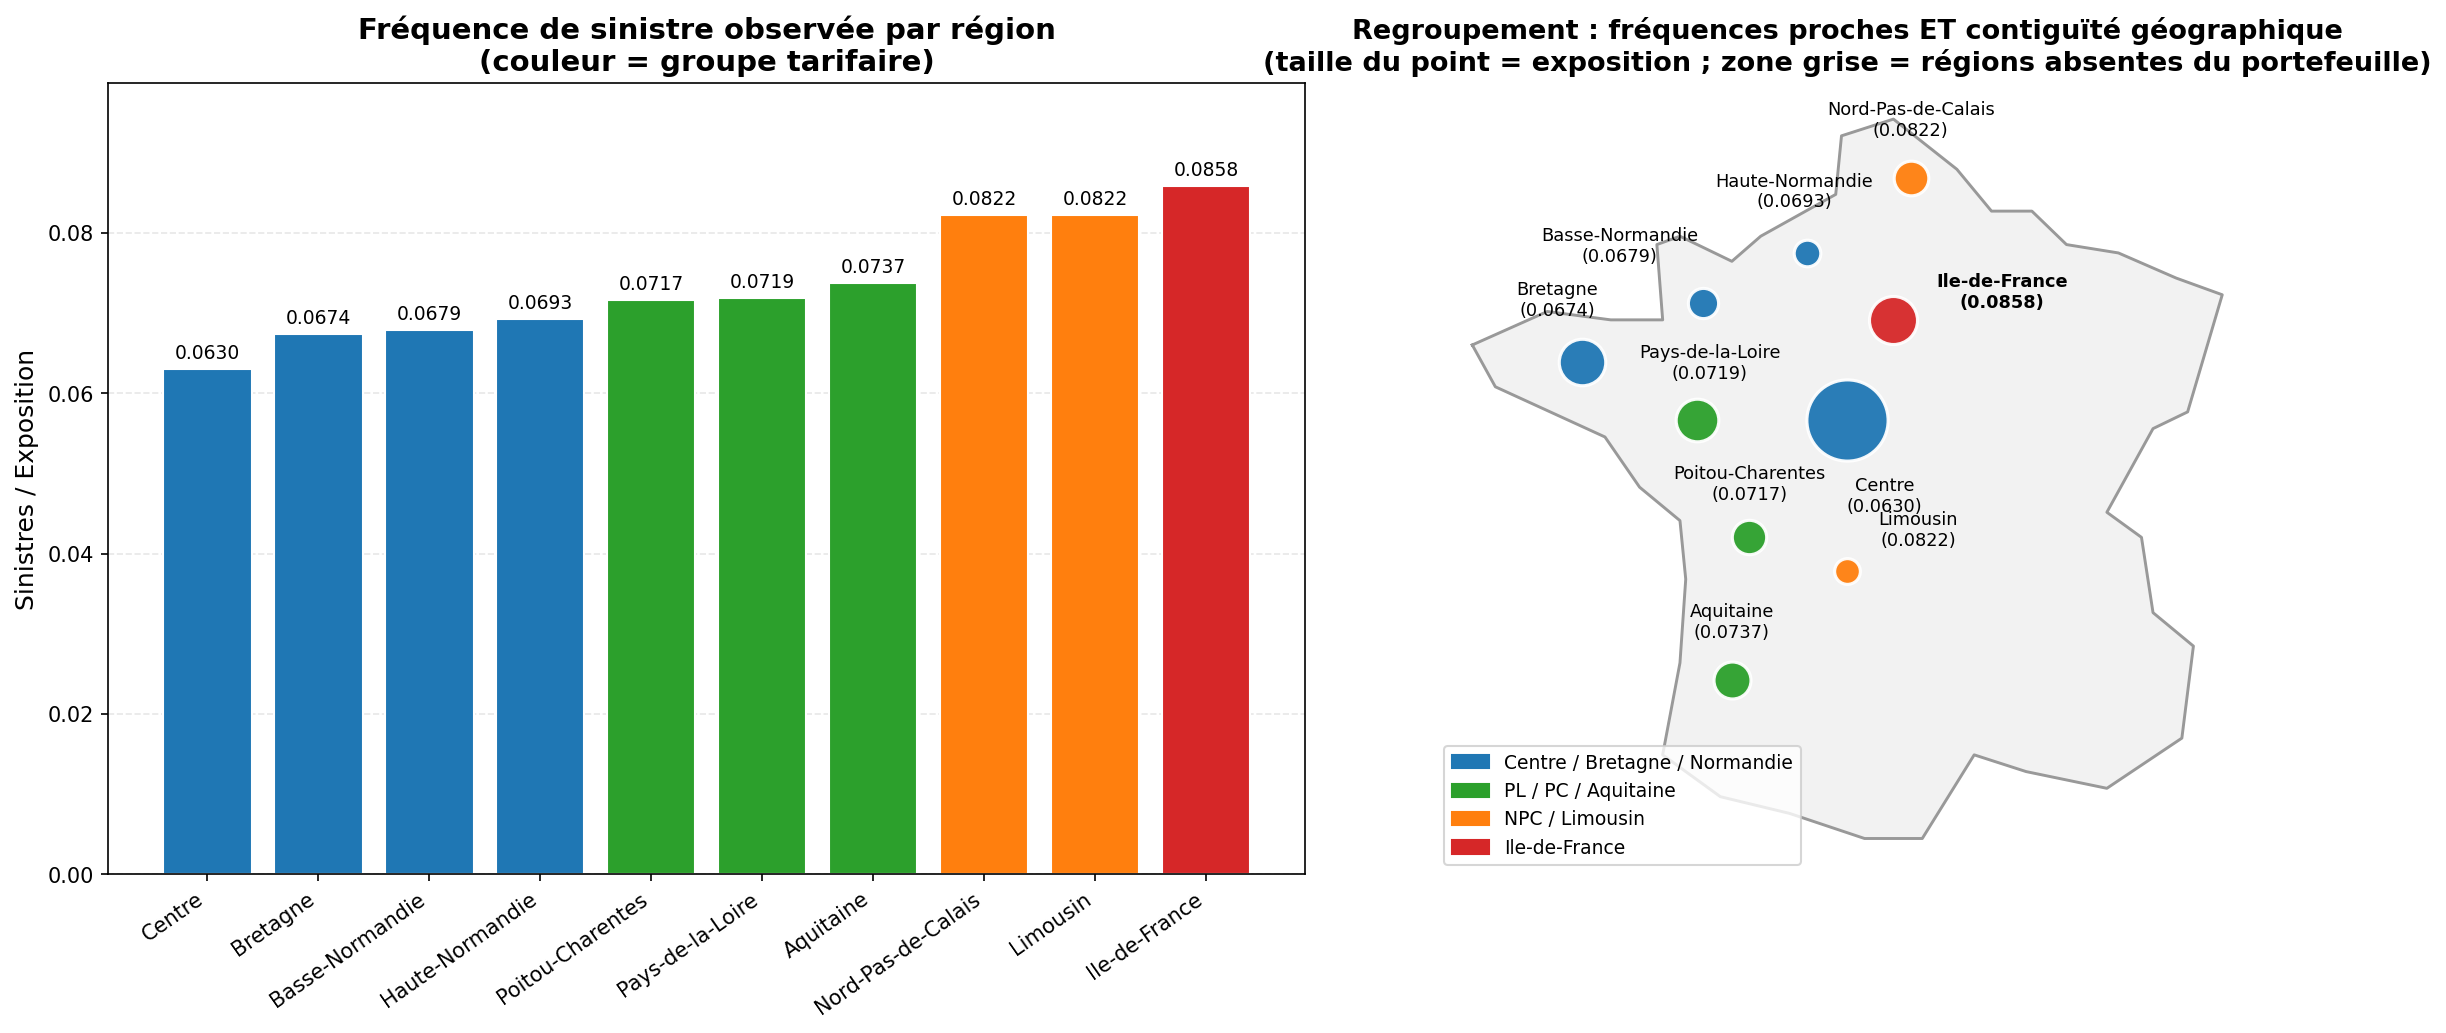
\includegraphics[width=\textwidth]{region_grouping.png}
\caption{Regroupement des régions en quatre zones tarifaires. À gauche : fréquence de sinistre observée par région, colorée par zone. À droite : carte schématique montrant la contiguïté géographique des zones (taille des points proportionnelle à l'exposition).}
\label{fig:regions}
\end{figure}

\subsection{Discrétisation des variables continues}

Les variables continues sont discrétisées en classes de quantiles, apprises sur le train uniquement puis appliquées telles quelles au test (les bornes extrêmes étant ouvertes pour absorber toute valeur hors de l'intervalle d'apprentissage) :

\begin{table}[H]
\centering
\caption{Classes tarifaires issues de la discrétisation par quantiles}
\begin{tabular}{llrr}
\toprule
Variable & Classe & Borne inf. & Borne sup. \\
\midrule
CarAge (2 classes) & classe 1 & 0 & 7 \\
 & classe 2 & 7 & 100 \\
\midrule
DriverAge (5 classes) & classe 1 & 18 & 32 \\
 & classe 2 & 32 & 40 \\
 & classe 3 & 40 & 48 \\
 & classe 4 & 48 & 57 \\
 & classe 5 & 57 & 99 \\
\midrule
$\log$(Density) (5 classes) & classe 1 & 0{,}69 & 3{,}93 \\
 & classe 2 & 3{,}93 & 5{,}06 \\
 & classe 3 & 5{,}06 & 6{,}31 \\
 & classe 4 & 6{,}31 & 7{,}78 \\
 & classe 5 & 7{,}78 & 10{,}20 \\
\bottomrule
\end{tabular}
\end{table}

\paragraph{Pourquoi discrétiser ?} Un GLM impose une forme fonctionnelle : entrer \texttt{DriverAge} linéairement supposerait un effet log-linéaire de l'âge sur la fréquence, ce que dément l'exploration (risque élevé chez les jeunes, plateau, remontée éventuelle aux grands âges). La discrétisation en classes capture ces non-linéarités sans hypothèse de forme, au prix d'effets en escalier --- et produit directement les cases d'une grille tarifaire commercialisable. \texttt{Density} est préalablement passée au logarithme pour que les quantiles découpent une échelle pertinente.

% =====================================================================
\section{Modèles GLM : résultats}
% =====================================================================

\subsection{Modèle de fréquence}

Le modèle retenu inclut les sept variables tarifaires :
\[
\texttt{ClaimNb} \sim \texttt{Power} + \texttt{Brand} + \texttt{Region} + \texttt{DriverAge} + \texttt{CarAge} + \texttt{Gas} + \texttt{Density}
\]
avec offset $\log(\texttt{Exposure})$, soit 24 paramètres pour un AIC de 107\,898. Sur le test : MAE $= 0{,}0753$, RMSE $= 0{,}2065$. Ces métriques ponctuelles sont dominées par la masse de polices sans sinistre ; l'évaluation discriminante pertinente (déviance de Poisson, Gini) est présentée en section~\ref{sec:compare}.

\subsection{Modèle de sévérité et sélection de variables}

Une recherche exhaustive sur les $\sum_{k=2}^{7}\binom{7}{k} = 120$ sous-ensembles de variables, classés par AIC, a été conduite pour le modèle Gamma. Le modèle \textbf{complet à sept variables} minimise l'AIC (254\,623, contre 254\,709 pour le meilleur modèle à six variables, sans \texttt{CarAge}) : toutes les variables apportent une information de sévérité qui justifie leur coût en paramètres. Sur le test : MAE $= 1\,944$~\eur, RMSE $= 8\,432$~\eur{} --- l'ordre de grandeur du RMSE, comparable à la sévérité moyenne elle-même, illustre déjà la difficulté intrinsèque de prédire les montants individuels en présence de queue épaisse.

\subsection{Prime pure et équilibre global}

La prime pure standard $\widehat{N} \times \widehat{S}$ donne sur le test :
\begin{table}[H]
\centering
\caption{Équilibre du tarif GLM standard sur le test (82\,634 polices)}
\begin{tabular}{lr}
\toprule
Charge observée & 6{,}38~M\eur \\
Prime totale prédite & 6{,}91~M\eur \\
Ratio S/P & 0{,}9234 \\
Prime pure moyenne & 83{,}64~\eur \\
\bottomrule
\end{tabular}
\end{table}

Le S/P de 0{,}92 traduit une légère surtarification sur cet échantillon de test --- l'équilibre exact n'est garanti par le GLM que sur le train ; l'écart au test reflète l'aléa d'échantillonnage de la charge, très volatile du fait des graves.

% =====================================================================
\section{Moteur tarifaire : relativités et grille}
% =====================================================================

Le tarif multiplicatif est reconstruit à partir des coefficients des deux GLM. La prime de référence (profil de référence sur toutes les variables, exposition pleine) s'établit à \textbf{188{,}06~\eur}.

\begin{table}[H]
\centering
\caption{Relativités du tarif (référence $=1$ ; combiné $=$ fréquence \texttimes{} sévérité)}
\small
\begin{tabular}{llrrr}
\toprule
Variable & Modalité & Rel. fréq. & Rel. sév. & Rel. combinée \\
\midrule
Power & d (réf.) & 1{,}000 & 1{,}000 & 1{,}000 \\
 & f & 1{,}106 & 1{,}387 & 1{,}534 \\
 & h & 1{,}132 & 1{,}096 & 1{,}241 \\
 & i\_j\_k & 1{,}243 & 1{,}628 & \textbf{2{,}024} \\
 & l\_o\_g & 1{,}084 & 1{,}157 & 1{,}254 \\
 & m\_e & 1{,}102 & 1{,}018 & 1{,}122 \\
 & n & 1{,}266 & 1{,}210 & 1{,}532 \\
\midrule
Brand & Japonaises/coréennes (réf.) & 1{,}000 & 1{,}000 & 1{,}000 \\
 & MCB\_Fiat & 1{,}299 & 0{,}721 & 0{,}936 \\
 & Opel/GM/Ford & 1{,}358 & 0{,}671 & 0{,}911 \\
 & RNC\_other & 1{,}193 & 0{,}839 & 1{,}001 \\
 & VW/Audi/Skoda/Seat & 1{,}253 & 0{,}851 & 1{,}067 \\
\midrule
Region & Centre/Bretagne/Norm. (réf.) & 1{,}000 & 1{,}000 & 1{,}000 \\
 & Île-de-France & 1{,}091 & 0{,}775 & 0{,}846 \\
 & NPC/Limousin & 1{,}116 & 0{,}735 & 0{,}820 \\
 & PL/PC/Aquitaine & 1{,}061 & 0{,}778 & 0{,}825 \\
\midrule
DriverAge & 18--32 ans (réf.) & 1{,}000 & 1{,}000 & 1{,}000 \\
 & 32--40 ans & 0{,}676 & 0{,}700 & 0{,}473 \\
 & 40--48 ans & 0{,}772 & 0{,}625 & 0{,}483 \\
 & 48--57 ans & 0{,}736 & 0{,}671 & 0{,}494 \\
 & 57--99 ans & 0{,}643 & 0{,}697 & \textbf{0{,}448} \\
\midrule
CarAge & 0--7 ans (réf.) & 1{,}000 & 1{,}000 & 1{,}000 \\
 & 7 ans et $+$ & 0{,}958 & 1{,}023 & 0{,}981 \\
\midrule
Gas & Diesel (réf.) & 1{,}000 & 1{,}000 & 1{,}000 \\
 & Essence & 0{,}852 & 1{,}114 & 0{,}949 \\
\midrule
Density & classe 1 (réf.) & 1{,}000 & 1{,}000 & 1{,}000 \\
 & classe 2 & 1{,}170 & 0{,}970 & 1{,}134 \\
 & classe 3 & 1{,}284 & 0{,}941 & 1{,}208 \\
 & classe 4 & 1{,}533 & 0{,}822 & 1{,}260 \\
 & classe 5 & 1{,}716 & 0{,}815 & \textbf{1{,}398} \\
\bottomrule
\end{tabular}
\label{tab:relativites}
\end{table}

\paragraph{Lecture actuarielle.} Trois enseignements ressortent de la table~\ref{tab:relativites} et justifient a posteriori la décomposition fréquence/sévérité :

\begin{itemize}
    \item \textbf{Des effets opposés qui se compensent.} Pour la marque, la région, le carburant et la densité, fréquence et sévérité jouent en sens \emph{contraires}. L'Île-de-France sinistre plus souvent ($+9\,\%$) mais moins cher ($-23\,\%$) --- typique d'une sinistralité urbaine de petits chocs matériels --- pour un effet net de $-15\,\%$. Un modèle qui n'observerait que le coût total manquerait cette structure.
    \item \textbf{L'âge du conducteur est le facteur dominant} : les 18--32 ans paient plus du double de toutes les autres classes (relativités combinées de 0{,}45 à 0{,}49), sous le double effet d'une fréquence et d'une sévérité plus élevées.
    \item \textbf{La densité est le second facteur} : $+40\,\%$ entre zones les moins et les plus denses, porté par la fréquence ($+72\,\%$) et amorti par la sévérité ($-19\,\%$).
\end{itemize}

À titre d'illustration, la grille croisée Puissance \texttimes{} Marque (profil fixé par ailleurs) s'étend de 99{,}90~\eur{} (puissance \texttt{d}, Opel/GM/Ford) à 236{,}78~\eur{} (puissance \texttt{i\_j\_k}, VW/Audi/Skoda/Seat), soit un rapport de 2{,}4 sur ces deux seuls axes (grille complète en annexe~\ref{annexe:grille}).

% =====================================================================
\section{Traitement des sinistres graves}
\label{sec:graves}
% =====================================================================

\subsection{Problématique}

Un GLM Gamma ajusté sur données brutes est otage de sa queue : les quelques sinistres à plusieurs centaines de milliers d'euros tirent les coefficients de manière erratique, et leur affectation aux modalités du hasard (un grave survenu en zone rurale ne dit rien du risque rural). La réponse actuarielle standard sépare le risque en deux composantes :
\begin{equation}
    \text{Prime pure} \;=\;
    \underbrace{\mathbb{E}[N] \times \mathbb{E}[S \wedge M_1]}_{\text{composante attritionnelle, segmentée}}
    \;+\;
    \underbrace{\mathbb{E}[N] \times p_{\text{atyp}} \times \mathbb{E}[(S - M_1)^+ \mid S > M_1]}_{\text{chargement atypique, mutualisé}}
\end{equation}
La composante attritionnelle (sinistres écrêtés au seuil $M_1$) reste finement segmentée par GLM ; l'excédent des graves, non segmentable, est mutualisé sur tout le portefeuille au prorata de la fréquence prédite.

\subsection{Choix du seuil}

La Mean Excess Function empirique $e(u) = \mathbb{E}[X - u \mid X > u]$ (figure \texttt{mean\_excess\_function}) présente le comportement croissant caractéristique d'une queue épaisse de type Pareto. Le seuil est fixé au quantile 99{,}5\,\% de la charge par police :
\begin{table}[H]
\centering
\caption{Caractéristiques du seuil et des sinistres graves (train)}
\begin{tabular}{lr}
\toprule
Seuil $M_1$ (quantile 99{,}5\,\%) & 40\,107~\eur \\
Polices atypiques & 62 (0{,}51\,\% des polices sinistrées) \\
Coût moyen d'une police atypique & 148\,823~\eur \\
Excédent moyen au-delà de $M_1$ & 108\,716~\eur \\
\bottomrule
\end{tabular}
\end{table}

Ce choix arbitre entre deux risques : un seuil trop bas écrête de l'information segmentable ; un seuil trop haut laisse des montants déstabilisants dans le GLM. Avec 62 observations au-delà du seuil, l'excédent moyen reste estimable tout en purgeant le GLM attritionnel de ses valeurs extrêmes.

\subsection{Calibrage du chargement}

Le chargement par sinistre est défini par :
\begin{equation}
    \text{chargement} \;=\; p_{\text{atyp}} \times \overline{\text{excédent}}
    \;=\; \frac{n_{\text{polices atypiques}}}{n_{\text{sinistres total}}} \times 108\,716~\text{\eur}
    \;=\; 523{,}93~\text{\eur}.
\end{equation}

La définition de $p_{\text{atyp}}$ mérite attention : le seuil s'appliquant à la charge \emph{totale par police}, chaque police atypique correspond à \emph{une} occurrence d'excédent, d'où un numérateur en nombre de polices. Cette convention garantit une propriété de \textbf{reconstruction exacte} : sur le train, la somme des chargements égale exactement l'excédent total écrêté. Une variante tentante --- pondérer $p_{\text{atyp}}$ par le nombre de sinistres des polices atypiques --- surchargerait le tarif de 16\,\%, les polices atypiques comptant en moyenne 1{,}16 sinistre.

\subsection{Résultats de la prime à deux composantes}

\begin{table}[H]
\centering
\caption{Comparaison des approches sur le test}
\begin{tabular}{lrr}
\toprule
Approche & Prime moyenne & Ratio S/P \\
\midrule
GLM standard (sans traitement des graves) & 83{,}64~\eur & 0{,}9234 \\
Deux composantes (écrêté $+$ chargement) & 85{,}25~\eur & 0{,}9060 \\
Loading simple (non écrêté $+$ chargement) & 104{,}11~\eur & 0{,}7419 \\
\bottomrule
\end{tabular}
\label{tab:sp2comp}
\end{table}

La sévérité attritionnelle prédite (1\,677~\eur{} en moyenne) est nettement inférieure à la sévérité brute (2\,155~\eur) : l'écrêtement remplit son office. Le chargement atypique représente en moyenne 24\,\% de la prime à deux composantes --- un quart du tarif couvre un demi-pour-cent des sinistres, illustration frappante du poids de la queue.

La ligne \og loading simple \fg{} de la table~\ref{tab:sp2comp} est conservée à dessein comme \textbf{contre-exemple pédagogique} : ajouter un chargement à une prime dont la sévérité n'a \emph{pas} été écrêtée double-compte les graves (ils sont dans la sévérité \emph{et} dans le chargement), d'où une surtarification de 25\,\% (S/P de 0{,}74). L'écrêtement et le chargement forment un tout indissociable.

% =====================================================================
\section{Approches Machine Learning}
% =====================================================================

\subsection{Motivation et principes de rigueur}

Le GLM impose additivité (sur l'échelle log) et effets en escalier ; un gradient boosting (LightGBM) apprend librement non-linéarités et interactions. Mais la comparaison n'est équitable que si le ML respecte les mêmes contraintes actuarielles que le GLM. Quatre principes structurent notre implémentation :

\paragraph{1. Traitement correct de l'exposition.} L'équivalent du GLM Poisson avec offset s'obtient en régressant le \emph{taux} $\texttt{ClaimNb}/\texttt{Exposure}$ avec l'objectif Poisson et un poids égal à l'exposition. Le modèle prédit alors une fréquence annuelle, multipliée par l'exposition en prédiction --- sans quoi les échelles de fréquence GLM et ML seraient incomparables.

\paragraph{2. Early stopping.} Plutôt qu'un nombre d'arbres fixé a priori (source de sur-apprentissage silencieux), chaque modèle part de 2\,000 arbres avec arrêt anticipé sur un jeu de validation (20\,\% du train), la métrique d'arrêt étant la déviance de la loi correspondante. Les données choisissent la complexité : 235 arbres pour la fréquence, 153 pour le Tweedie --- et, résultat remarquable, \textbf{3 arbres seulement pour la sévérité}.

\paragraph{3. Écrêtement identique au GLM.} La sévérité LightGBM est entraînée sur la sévérité écrêtée au même seuil (quantile 99{,}5\,\%), avec le même chargement atypique et la même pondération par \texttt{ClaimNb}. Un GBM ne peut pas plus qu'un GLM apprendre une queue de Pareto sur 62 observations.

\paragraph{4. Contraintes de monotonie.} La fréquence est contrainte à croître avec la densité de population. Un tarif présentant des inversions locales --- une prime qui baisse quand le risque monte --- serait commercialement et réglementairement indéfendable ; la contrainte agit de surcroît comme régularisation.

\subsection{Recalage global}

Contrairement au GLM Poisson, un GBM ne garantit aucun équilibre agrégé. Un facteur multiplicatif unique est donc appliqué pour forcer S/P $= 1$ sur le train. Les facteurs obtenus sont instructifs : \textbf{1{,}0003} pour la décomposition fréquence \texttimes{} sévérité écrêtée (quasi équilibrée par construction, validant la chaîne écrêtement $+$ chargement) contre \textbf{1{,}2930} pour le Tweedie brut, qui sous-tarife spontanément de 29\,\% --- le recalage n'est pas un raffinement optionnel mais une étape indispensable.

\subsection{Modèle Tweedie direct}

En complément de la décomposition, un modèle unique est ajusté sur la charge annuelle par police. La loi Tweedie de paramètre de variance $p \in (1, 2)$ est une loi Poisson composée Gamma : masse de probabilité en zéro (pas de sinistre) et distribution continue positive sinon --- exactement la structure d'une charge de sinistres. Avec $p = 1{,}5$ et pondération par l'exposition, le modèle apprend sur les 413\,169 polices (contre 12\,249 polices sinistrées pour le modèle de sévérité) et élimine tout risque d'incohérence à l'assemblage de deux modèles séparés.

% =====================================================================
\section{Comparaison des quatre tarifs}
\label{sec:compare}
% =====================================================================

\subsection{Le choix des métriques}

Le MAE et le RMSE sont inadaptés à ce problème : 96\,\% des polices n'ont aucun sinistre, si bien qu'un modèle prédisant zéro partout obtient un excellent MAE de fréquence. L'évaluation repose donc sur :
\begin{itemize}
    \item la \textbf{déviance de Poisson} (fréquence) : la métrique de vraisemblance propre au comptage ;
    \item l'\textbf{indice de Gini} sur la courbe de Lorenz ordonnée (polices triées par prime prédite croissante, part cumulée des sinistres en ordonnée) : mesure du pouvoir de segmentation, la métrique reine pour comparer des tarifs ;
    \item le \textbf{ratio S/P} : calibration globale ;
    \item les \textbf{tables de lift} par décile de prime prédite : calibration locale.
\end{itemize}

\subsection{Résultats}

\begin{table}[H]
\centering
\caption{Comparaison finale sur le test (82\,634 polices alignées)}
\begin{tabular}{lccc}
\toprule
Modèle & Déviance Poisson & Gini & S/P \\
\midrule
GLM fréquence \texttimes{} sévérité & 0{,}2582 & \textbf{0{,}191} & 0{,}923 \\
GLM deux composantes & 0{,}2582 & 0{,}180 & 0{,}906 \\
ML fréquence \texttimes{} sévérité (écrêté, recalé) & \textbf{0{,}2566} & 0{,}183 & 0{,}907 \\
Tweedie direct (recalé) & --- & 0{,}174 & 0{,}913 \\
\bottomrule
\end{tabular}
\label{tab:final}
\end{table}

\begin{figure}[H]
\centering
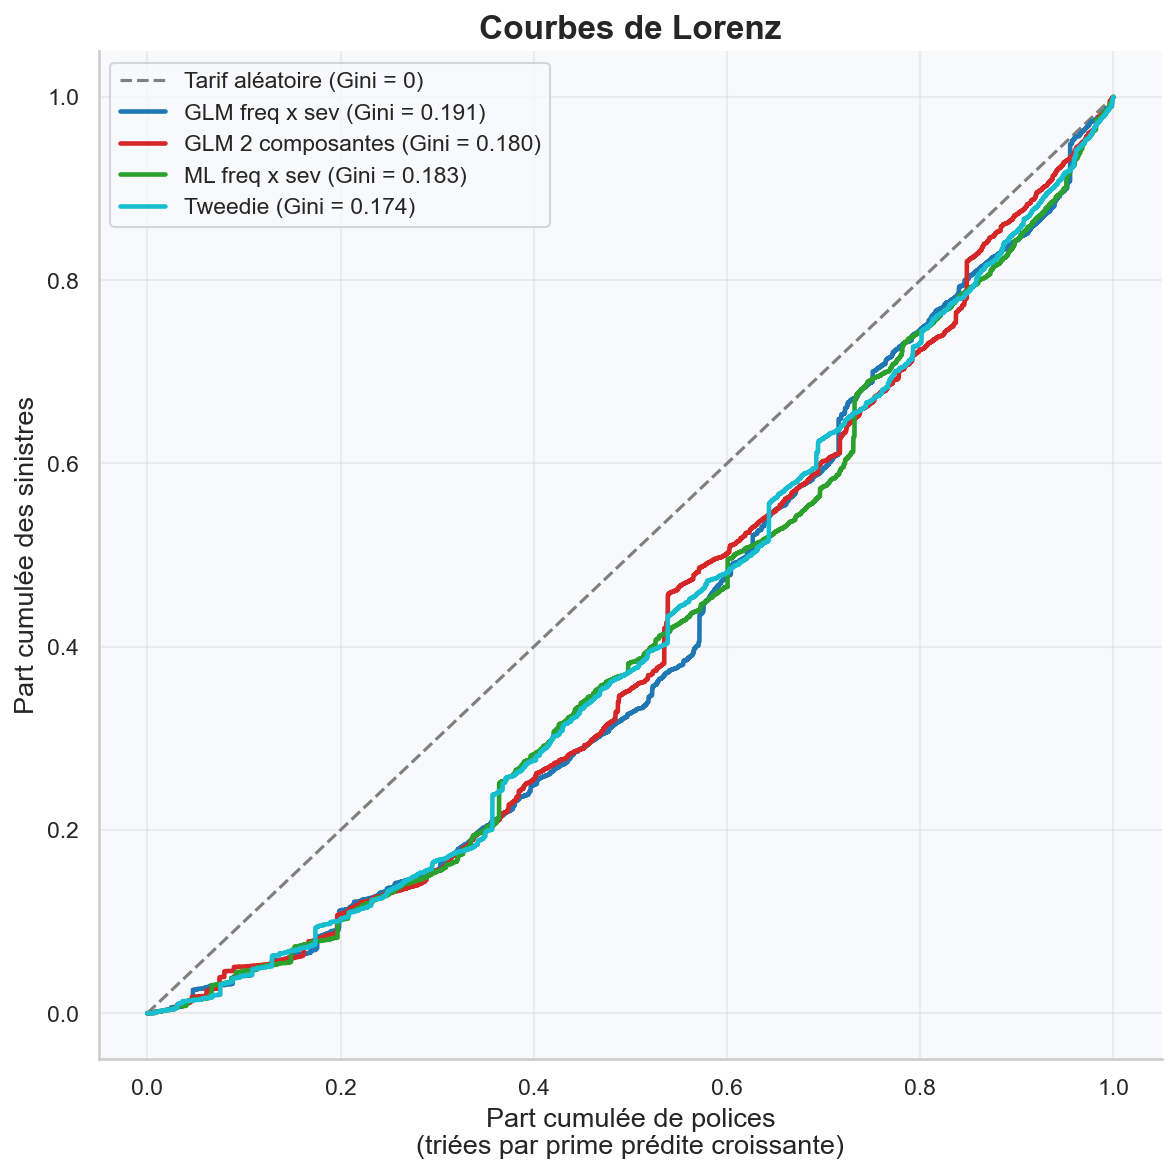
\includegraphics[width=0.62\textwidth]{lorenz_curves.png}
\caption{Courbes de Lorenz des quatre tarifs sur le test.}
\end{figure}

\paragraph{Le GLM tient tête au machine learning.} C'est le résultat central de la comparaison. Le LightGBM améliore la déviance de fréquence ($0{,}2566$ contre $0{,}2582$, gain modeste), mais le GLM conserve le meilleur Gini. Sur un portefeuille de sept variables aux effets essentiellement additifs, la marge de manœuvre du boosting --- capturer interactions et non-linéarités --- trouve peu de matière. Ce constat, conforme à la littérature sur \texttt{freMTPL}, est précieux en pratique : le GLM offre l'interprétabilité réglementaire \emph{sans} sacrifice de performance mesurable ici.

\paragraph{La sévérité n'est presque pas segmentable.} L'early stopping du modèle de sévérité s'arrête après 3 arbres : au-delà de la moyenne, presque rien n'est généralisable dans les montants écrêtés. La segmentation des tarifs provient donc quasi exclusivement de la fréquence --- constat actuariel classique que le protocole rend ici visible et quantifié, là où 500 arbres fixés a priori l'auraient masqué sous du sur-apprentissage.

\subsection{Calibration locale et biais d'exposition}

\begin{figure}[H]
\centering
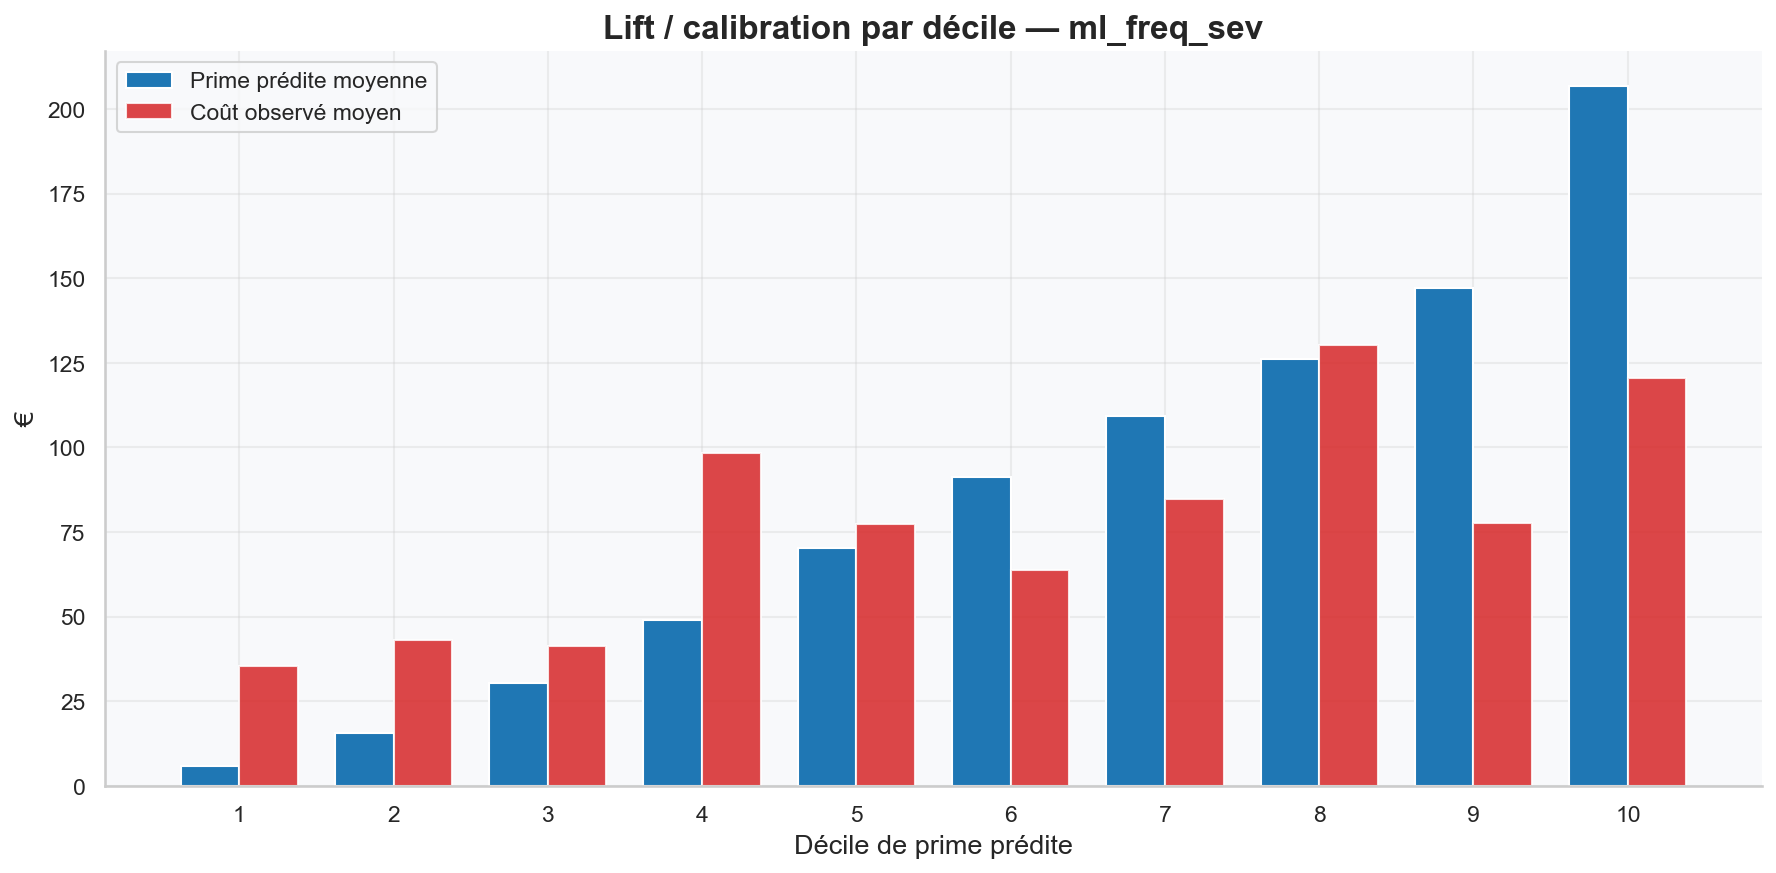
\includegraphics[width=0.75\textwidth]{lift_ml_freq_sev.png}
\caption{Table de lift du tarif ML : prime prédite vs coût observé par décile de prime prédite.}
\label{fig:lift}
\end{figure}

Les tables de lift révèlent un phénomène commun aux quatre tarifs : le premier décile de prime prédite présente un coût observé environ six fois supérieur à sa prime (35~\eur{} observés contre 6~\eur{} prédits pour le ML). L'explication tient à un biais structurel du jeu de données : \textbf{l'exposition est partiellement endogène au sinistre}. Une police résiliée à la suite d'un sinistre cumule mécaniquement une exposition courte \emph{et} un sinistre ; tout tarif proportionnel à l'exposition sous-tarife donc les polices courtes. Ce biais, documenté sur \texttt{freMTPL}, ne peut être corrigé par aucun choix de modèle --- il relève de la définition même de l'exposition et devrait, en contexte opérationnel, être traité en amont (exposition contractuelle plutôt qu'observée, ou modélisation de la résiliation).

Au-delà du premier décile, la calibration est convenable au centre de la distribution et le rapport observé/prédit décroît globalement le long des déciles, signe que les tarifs sur-étalent légèrement les primes par rapport au signal réellement présent --- conséquence directe de la faible segmentabilité de la sévérité.

\subsection{Interprétabilité des modèles ML}

L'analyse d'interprétabilité (figures \texttt{importance\_*}, \texttt{pdp\_*}, \texttt{shap\_*}) valide la cohérence actuarielle des modèles boostés :

\begin{itemize}
    \item l'\textbf{importance par gain} confirme la hiérarchie du GLM : âge du conducteur et densité dominent la fréquence ;
    \item les \textbf{partial dependence plots} de la fréquence reproduisent les formes attendues --- décroissance forte avec l'âge du conducteur, croissance monotone avec la densité (contrainte respectée), quasi-neutralité de l'âge du véhicule --- et permettent de vérifier qu'aucun effet appris n'est actuariellement aberrant ;
    \item les \textbf{valeurs SHAP} (TreeSHAP exact, calcul natif LightGBM, sur l'échelle du prédicteur logarithmique) fournissent la décomposition additive de chaque prime individuelle --- l'équivalent, police par police, de ce que la table des relativités offre au niveau du tarif.
\end{itemize}

\begin{figure}[H]
\centering
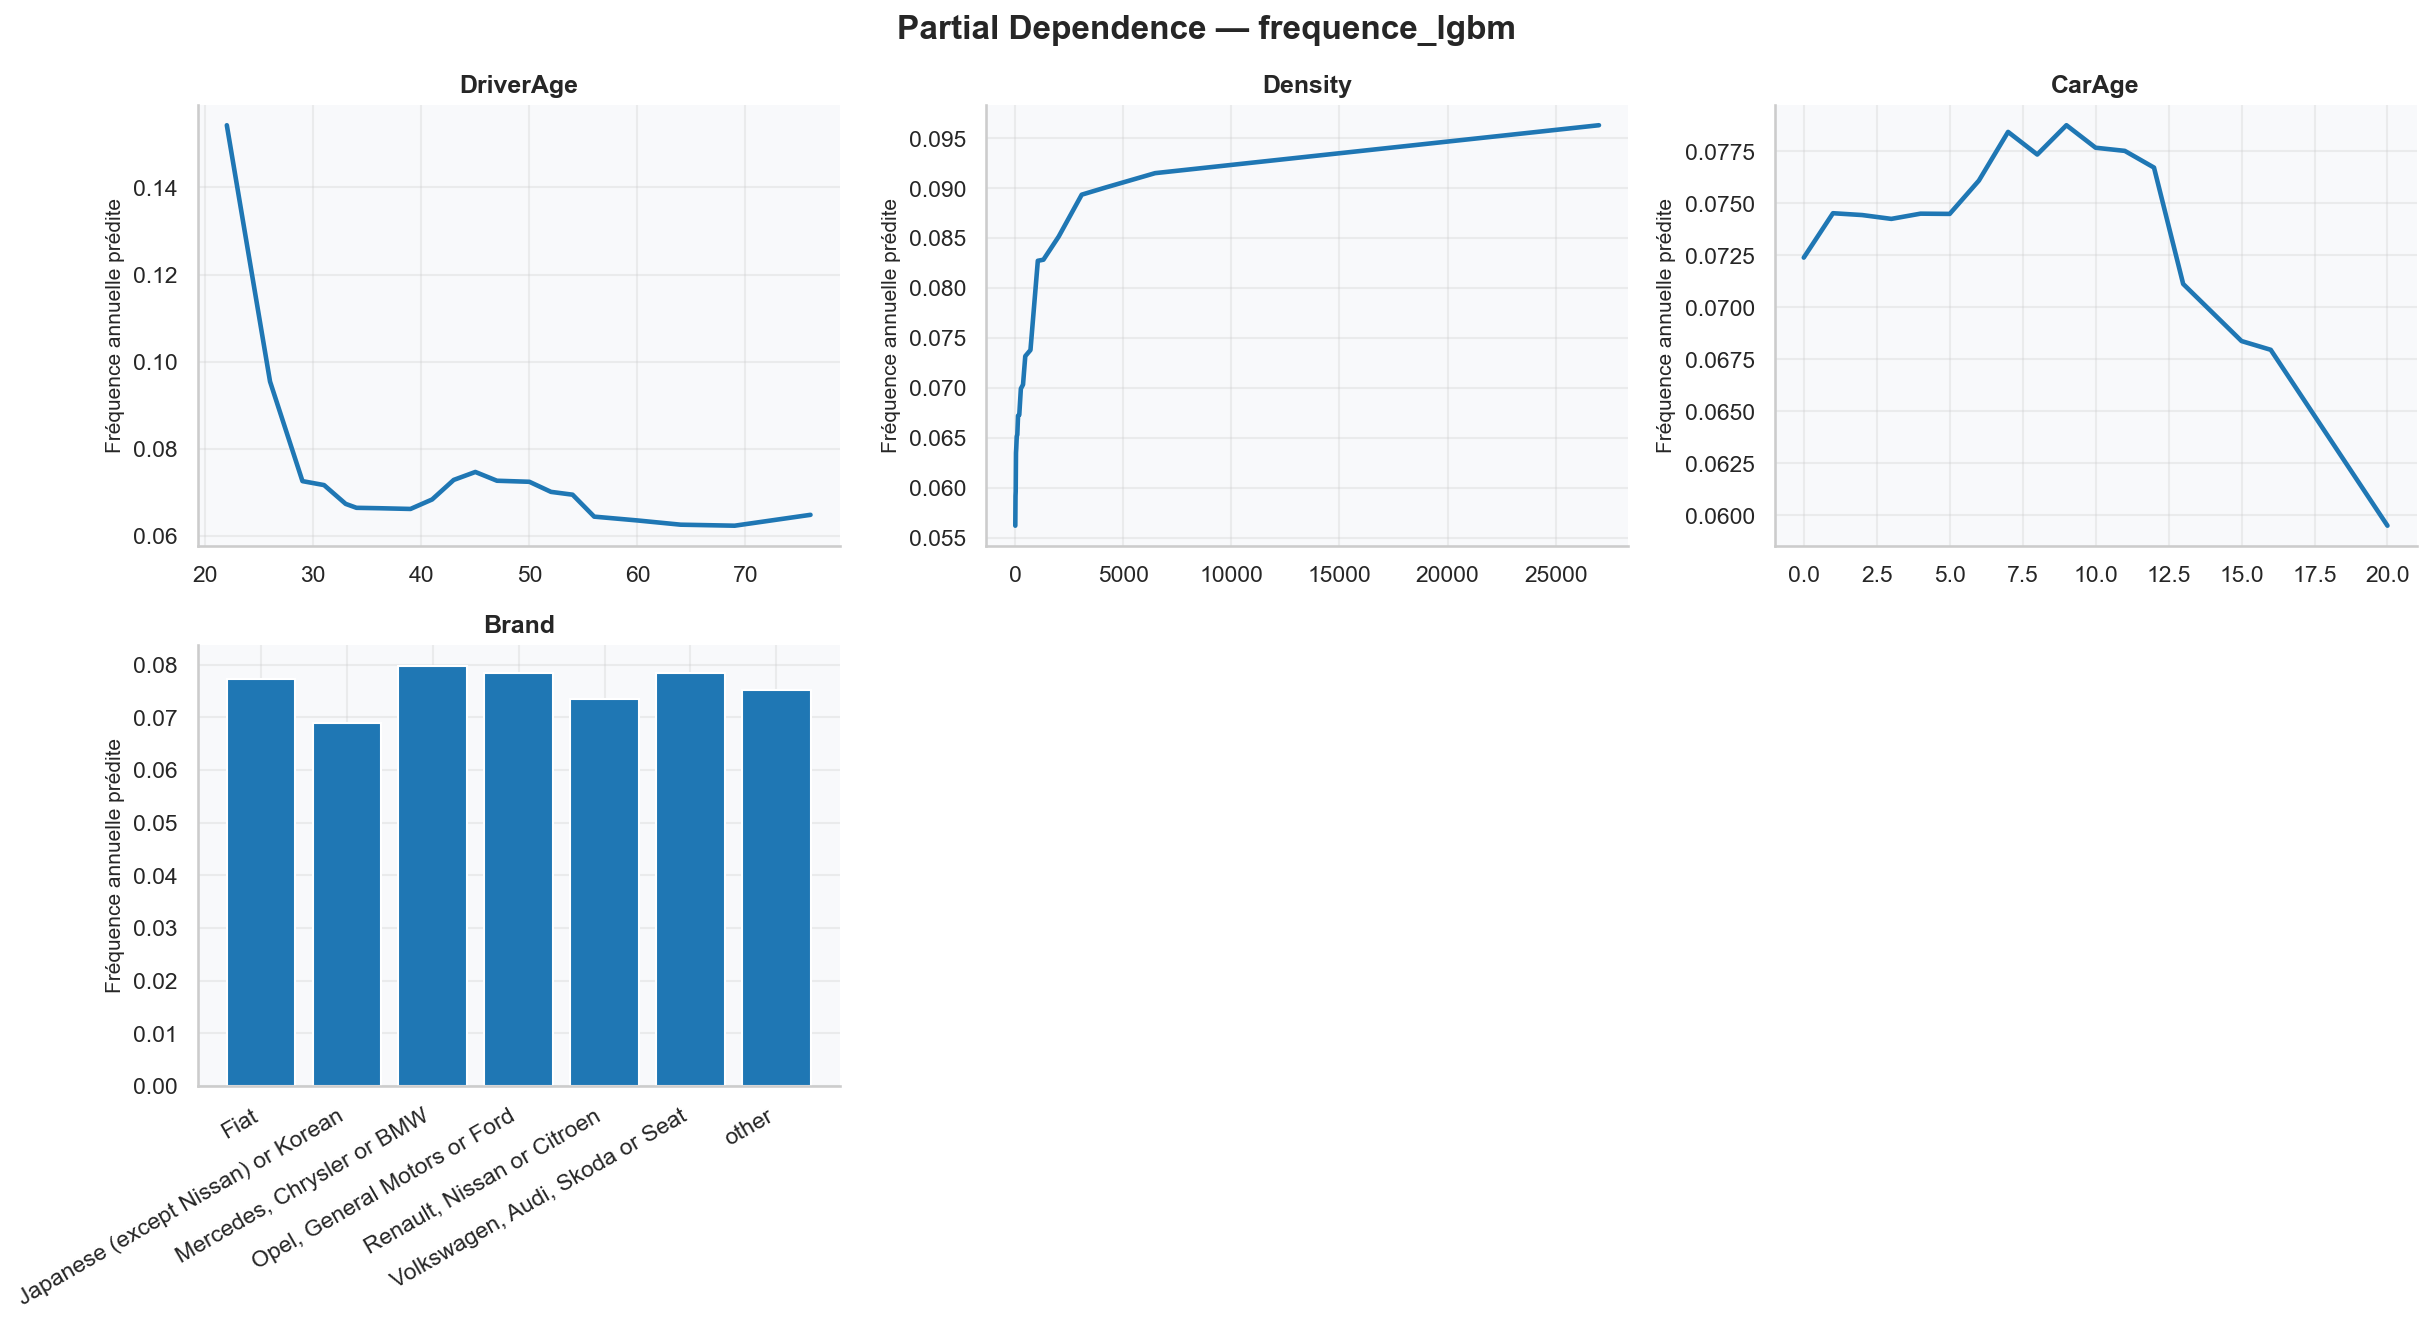
\includegraphics[width=\textwidth]{pdp_frequence_lgbm.png}
\caption{Partial dependence du modèle de fréquence LightGBM : effets marginaux moyens, à confronter aux relativités du GLM (table~\ref{tab:relativites}).}
\end{figure}

En pratique de marché, cette complémentarité s'exploite dans les deux sens : le GBM sert de \emph{détecteur} d'interactions et de non-linéarités manquées, que l'actuaire réinjecte ensuite dans le GLM tarifaire sous forme de termes croisés ou de nouveaux découpages de classes.

% =====================================================================
\section{Forces et limites des approches}
% =====================================================================

\begin{table}[H]
\centering
\caption{Synthèse comparative des trois familles de modèles}
\small
\begin{tabular}{p{3.2cm}p{3.6cm}p{3.6cm}p{3.6cm}}
\toprule
 & GLM freq \texttimes{} sév & GBM freq \texttimes{} sév & Tweedie direct \\
\midrule
Interprétabilité & Totale (relativités, grille multiplicative) & Indirecte (SHAP, PDP) & Indirecte (SHAP, PDP) \\
\addlinespace
Équilibre agrégé & Garanti sur le train (global et par modalité) & Recalage nécessaire (facteur 1{,}0003) & Recalage indispensable (facteur 1{,}29) \\
\addlinespace
Interactions, non-linéarités & À spécifier manuellement & Apprises automatiquement & Apprises automatiquement \\
\addlinespace
Données d'apprentissage sévérité & Polices sinistrées (12\,k) & Polices sinistrées (12\,k) & Tout le portefeuille (413\,k) \\
\addlinespace
Risque d'assemblage freq/sév & Oui (hyp. d'indépendance) & Oui & Non (modèle unique) \\
\addlinespace
Acceptabilité réglementaire & Standard de marché & À documenter & À documenter \\
\addlinespace
Performance observée (Gini) & \textbf{0{,}191} & 0{,}183 & 0{,}174 \\
\bottomrule
\end{tabular}
\end{table}

Sur ce portefeuille, la recommandation opérationnelle serait de \textbf{retenir le GLM à deux composantes comme tarif de production} (interprétable, équilibré, traitement explicite des graves) et de \textbf{conserver le GBM comme outil de contrôle} : surveillance des poches de risque mal capturées et détection d'interactions candidates à l'intégration dans le GLM.

% =====================================================================
\section{Limites et pistes d'amélioration}
% =====================================================================

\subsection{Limites identifiées}

\begin{enumerate}
    \item \textbf{Exposition endogène} : le biais du premier décile de lift (section~\ref{sec:compare}) affecte tous les modèles et ne peut être résolu qu'en amont des données.
    \item \textbf{Granularité police des graves} : le seuil $M_1$ s'applique à la charge totale par police et non au sinistre individuel ; une police peut franchir le seuil par accumulation de sinistres moyens. L'approximation est quantifiée (les polices atypiques comptent 1{,}16 sinistre en moyenne) mais une base au sinistre serait préférable.
    \item \textbf{Hypothèse d'indépendance fréquence--sévérité} : classique mais non testée ici ; les relativités opposées observées (Île-de-France : fréquence en hausse, sévérité en baisse) suggèrent une dépendance au niveau des facteurs de risque, capturée par les variables, mais une dépendance résiduelle reste possible.
    \item \textbf{Validation par découpage aléatoire unique} : pas de validation croisée complète du pipeline ni de validation temporelle (une seule année de données).
    \item \textbf{Gini modeste en absolu} ($\approx 0{,}18$) : avec sept variables tarifaires sans historique de conduite (bonus-malus, kilométrage, sinistralité passée), le plafond de segmentation atteignable est vite touché.
\end{enumerate}

\subsection{Pistes d'amélioration}

\paragraph{Court terme (données et modèles existants).}
\begin{itemize}
    \item optimiser le paramètre de variance Tweedie ($p$ balayé sur $[1{,}2 \,;\, 1{,}8]$ par validation croisée) plutôt que fixé à 1{,}5 ;
    \item recherche d'hyperparamètres systématique des GBM (Optuna) : \texttt{num\_leaves}, \texttt{min\_child\_samples}, régularisation L2 ;
    \item exploiter les PDP/SHAP du GBM pour enrichir le GLM d'interactions ciblées (par exemple âge \texttimes{} densité) et retester l'AIC ;
    \item étudier une modélisation de l'excédent des graves par loi de Pareto généralisée (théorie des valeurs extrêmes) au lieu de la moyenne empirique, pour stabiliser le chargement.
\end{itemize}

\paragraph{Moyen terme (méthodologie).}
\begin{itemize}
    \item validation croisée complète du pipeline (regroupements et discrétisations compris) pour mesurer la variance des relativités ;
    \item lissage géographique du zonier (modèles spatiaux, graphes de contiguïté) en remplacement du regroupement manuel des régions ;
    \item théorie de la crédibilité pour les modalités à faible exposition, en alternative aux regroupements ;
    \item modèle de résiliation pour corriger l'endogénéité de l'exposition.
\end{itemize}

\paragraph{Long terme (données).} L'essentiel du gain résiduel est dans les données plus que dans les modèles : historique de sinistralité individuelle (bonus-malus), kilométrage, usage du véhicule, données de conduite. Aucun raffinement algorithmique ne remplace une variable informative absente.

% =====================================================================
\section{Conclusion}
% =====================================================================

Ce projet a construit une chaîne de tarification complète et méthodologiquement rigoureuse : préparation des variables justifiée par l'exploration (regroupements sur double critère fréquence/géographie, discrétisation par quantiles), décomposition fréquence \texttimes{} sévérité par GLM avec les précautions d'usage (offset d'exposition, pondération de la sévérité, protocole anti-fuite), traitement des sinistres graves par écrêtement et chargement à reconstruction exacte, et confrontation loyale à deux approches de machine learning soumises aux mêmes contraintes actuarielles (exposition, écrêtement, recalage, monotonie).

Les résultats délivrent un message nuancé et utile : sur un portefeuille aux variables peu nombreuses et aux effets additifs, \textbf{le GLM demeure l'outil de production de référence} --- meilleur Gini, équilibre garanti, interprétabilité totale --- tandis que le machine learning apporte une validation indépendante, un léger gain en déviance de fréquence, et surtout un outillage d'exploration (SHAP, PDP, importance) qui renforce la confiance dans le tarif. Les deux constats structurels mis au jour --- la quasi-impossibilité de segmenter la sévérité au-delà de sa moyenne, et l'endogénéité de l'exposition au sinistre --- valent enfin comme mises en garde générales, indépendantes du choix de modèle.

\newpage
\appendix

% =====================================================================
\section{Grille tarifaire Puissance \texttimes{} Marque}
\label{annexe:grille}
% =====================================================================

Profil fixé : région Centre/Bretagne/Normandie, conducteur 40--48 ans, véhicule de moins de 7 ans, diesel, densité classe 3.

\begin{table}[H]
\centering
\caption{Prime pure (\eur) par croisement Puissance \texttimes{} Marque}
\small
\begin{tabular}{lrrrrr}
\toprule
 & Japon./cor. & MCB/Fiat & Opel/GM/Ford & RNC/other & VW/Audi/Skoda/Seat \\
\midrule
d & 109{,}69 & 102{,}68 & 99{,}90 & 109{,}77 & 116{,}99 \\
f & 168{,}24 & 157{,}48 & 153{,}23 & 168{,}36 & 179{,}44 \\
h & 136{,}16 & 127{,}44 & 124{,}01 & 136{,}25 & 145{,}22 \\
i\_j\_k & 222{,}01 & 207{,}81 & 202{,}20 & 222{,}17 & 236{,}78 \\
l\_o\_g & 137{,}55 & 128{,}75 & 125{,}27 & 137{,}64 & 146{,}70 \\
m\_e & 123{,}07 & 115{,}20 & 112{,}09 & 123{,}16 & 131{,}26 \\
n & 168{,}02 & 157{,}27 & 153{,}02 & 168{,}14 & 179{,}20 \\
\bottomrule
\end{tabular}
\end{table}

% =====================================================================
\section{Tables de lift complètes}
% =====================================================================

\begin{table}[H]
\centering
\caption{Lift par décile de prime prédite --- test (moyennes en \eur)}
\small
\begin{tabular}{c rr rr rr}
\toprule
 & \multicolumn{2}{c}{GLM} & \multicolumn{2}{c}{ML freq \texttimes{} sév} & \multicolumn{2}{c}{Tweedie} \\
\cmidrule(lr){2-3} \cmidrule(lr){4-5} \cmidrule(lr){6-7}
Décile & Prédit & Observé & Prédit & Observé & Prédit & Observé \\
\midrule
1  & 5{,}29   & 31{,}41  & 5{,}88   & 35{,}36  & 5{,}30   & 31{,}67 \\
2  & 14{,}74  & 55{,}22  & 15{,}69  & 42{,}99  & 14{,}38  & 47{,}83 \\
3  & 28{,}48  & 34{,}21  & 30{,}27  & 41{,}35  & 27{,}77  & 49{,}24 \\
4  & 46{,}34  & 71{,}64  & 49{,}02  & 98{,}41  & 44{,}85  & 84{,}33 \\
5  & 66{,}35  & 60{,}38  & 70{,}32  & 77{,}30  & 63{,}89  & 75{,}35 \\
6  & 85{,}94  & 115{,}38 & 91{,}23  & 63{,}84  & 82{,}78  & 83{,}14 \\
7  & 102{,}23 & 91{,}14  & 109{,}40 & 84{,}82  & 101{,}09 & 113{,}16 \\
8  & 119{,}21 & 116{,}09 & 126{,}09 & 130{,}27 & 120{,}68 & 80{,}18 \\
9  & 144{,}49 & 76{,}25  & 147{,}05 & 77{,}56  & 146{,}07 & 93{,}65 \\
10 & 223{,}39 & 120{,}68 & 206{,}78 & 120{,}50 & 239{,}50 & 113{,}85 \\
\bottomrule
\end{tabular}
\end{table}

La forte volatilité des coûts observés par décile ($\approx$ 8\,260 polices par décile, fréquence $\approx 7\,\%$, sévérité à queue épaisse : un seul sinistre de 500\,k\eur{} déplace la moyenne d'un décile de 60~\eur) rappelle que ces tables se lisent en tendance, non décile par décile.

% =====================================================================
\section{Environnement technique}
% =====================================================================

Pipeline Python modulaire : \texttt{pandas} / \texttt{numpy} (données), \texttt{statsmodels} (GLM), \texttt{LightGBM}~4.6 (gradient boosting, TreeSHAP natif), \texttt{scikit-learn} (protocole de validation), \texttt{matplotlib} / \texttt{seaborn} (visualisation). Code organisé en couches : \texttt{data/} (chargement, préparation), \texttt{features/} (discrétisation), \texttt{models/} (GLM, graves, ML, évaluation), \texttt{pricing/} (relativités, moteur tarifaire, grilles), \texttt{visualization/} (EDA, graves, ML). Reproductibilité assurée par graine fixe (42) et configuration centralisée (\texttt{config.py}).

\end{document}
